After applying all of the previously discussed cuts as a tuned from the 10$\%$ sample, we see the resulting $z$ vertex distribution as a function of corrected mass in Figure~\ref{fig:zVm_bl}.

\begin{figure}[htb]
  \centering
      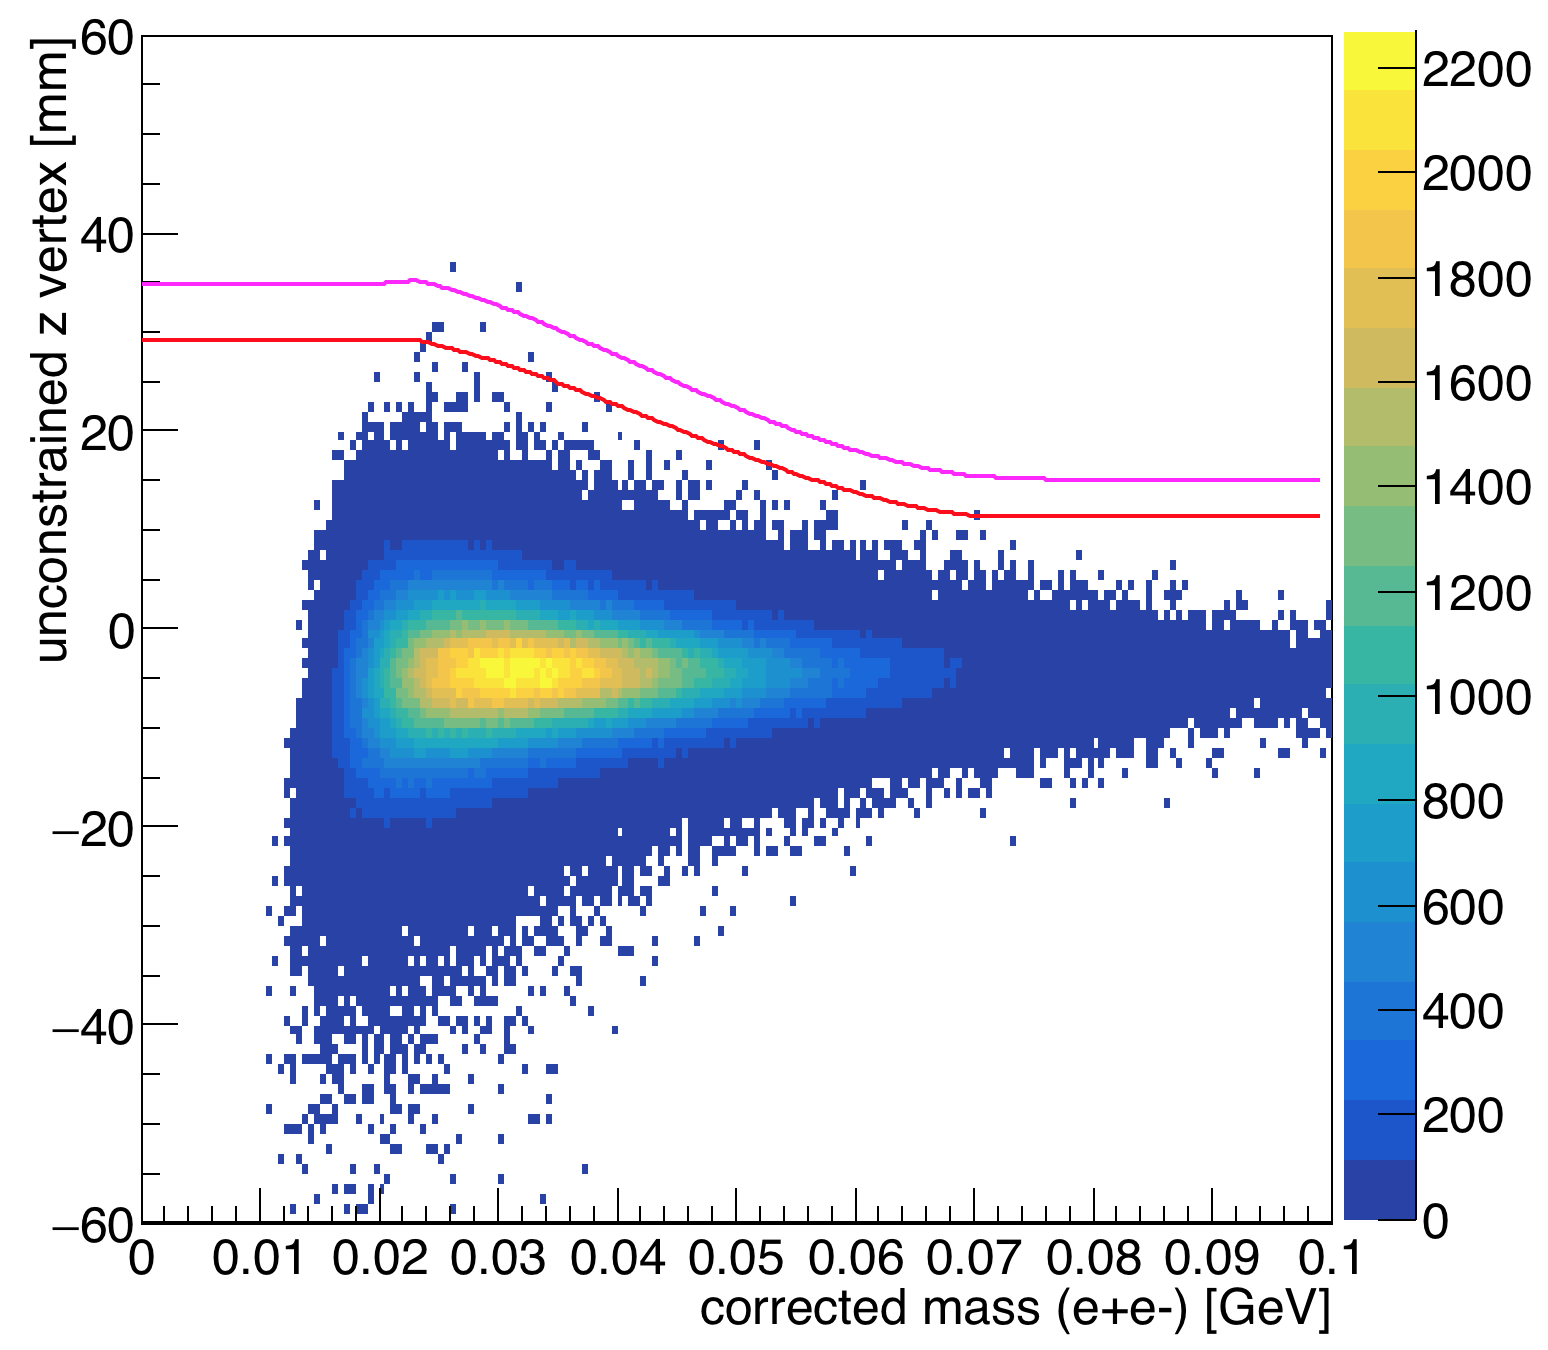
\includegraphics[width=0.75\textwidth]{pics/searching/zVm_bl_L1L1.png}
  \caption[Vertex position vs mass for the 10$\%$ L1L1 data]{The unconstrained $z$ vertex position is shown as a function of the corrected mass of the $e^+e^-$ pair. The $zCut$ as measured for this data is shown in red and corresponds to where there is less than 0.5 background event beyond. The projected $zCut$ for the full 100$\%$ data is shown in magenta. The relevant mass range used to fit $zCut$ is from 0.02-0.07~GeV based on measured statistics.}
  \label{fig:zVm_bl}
\end{figure} 

From this initial sample, we still see that there are 3 events in the high $z$ region that will be apparent in the full 100$\%$ dataset. In order to get a rough estimate from the contamination due to accidentals, vertices with cluster time differences greater than 3~ns and less than 9~ns were selected and the vertex distribution was studied. This time window was selected because SVT efficiency deteriorates outside of this and results in less reconstructed events. The accidental vertex distribution is shown in Figure~\ref{fig:zVm_acc}.

\begin{figure}[htb]
  \centering
      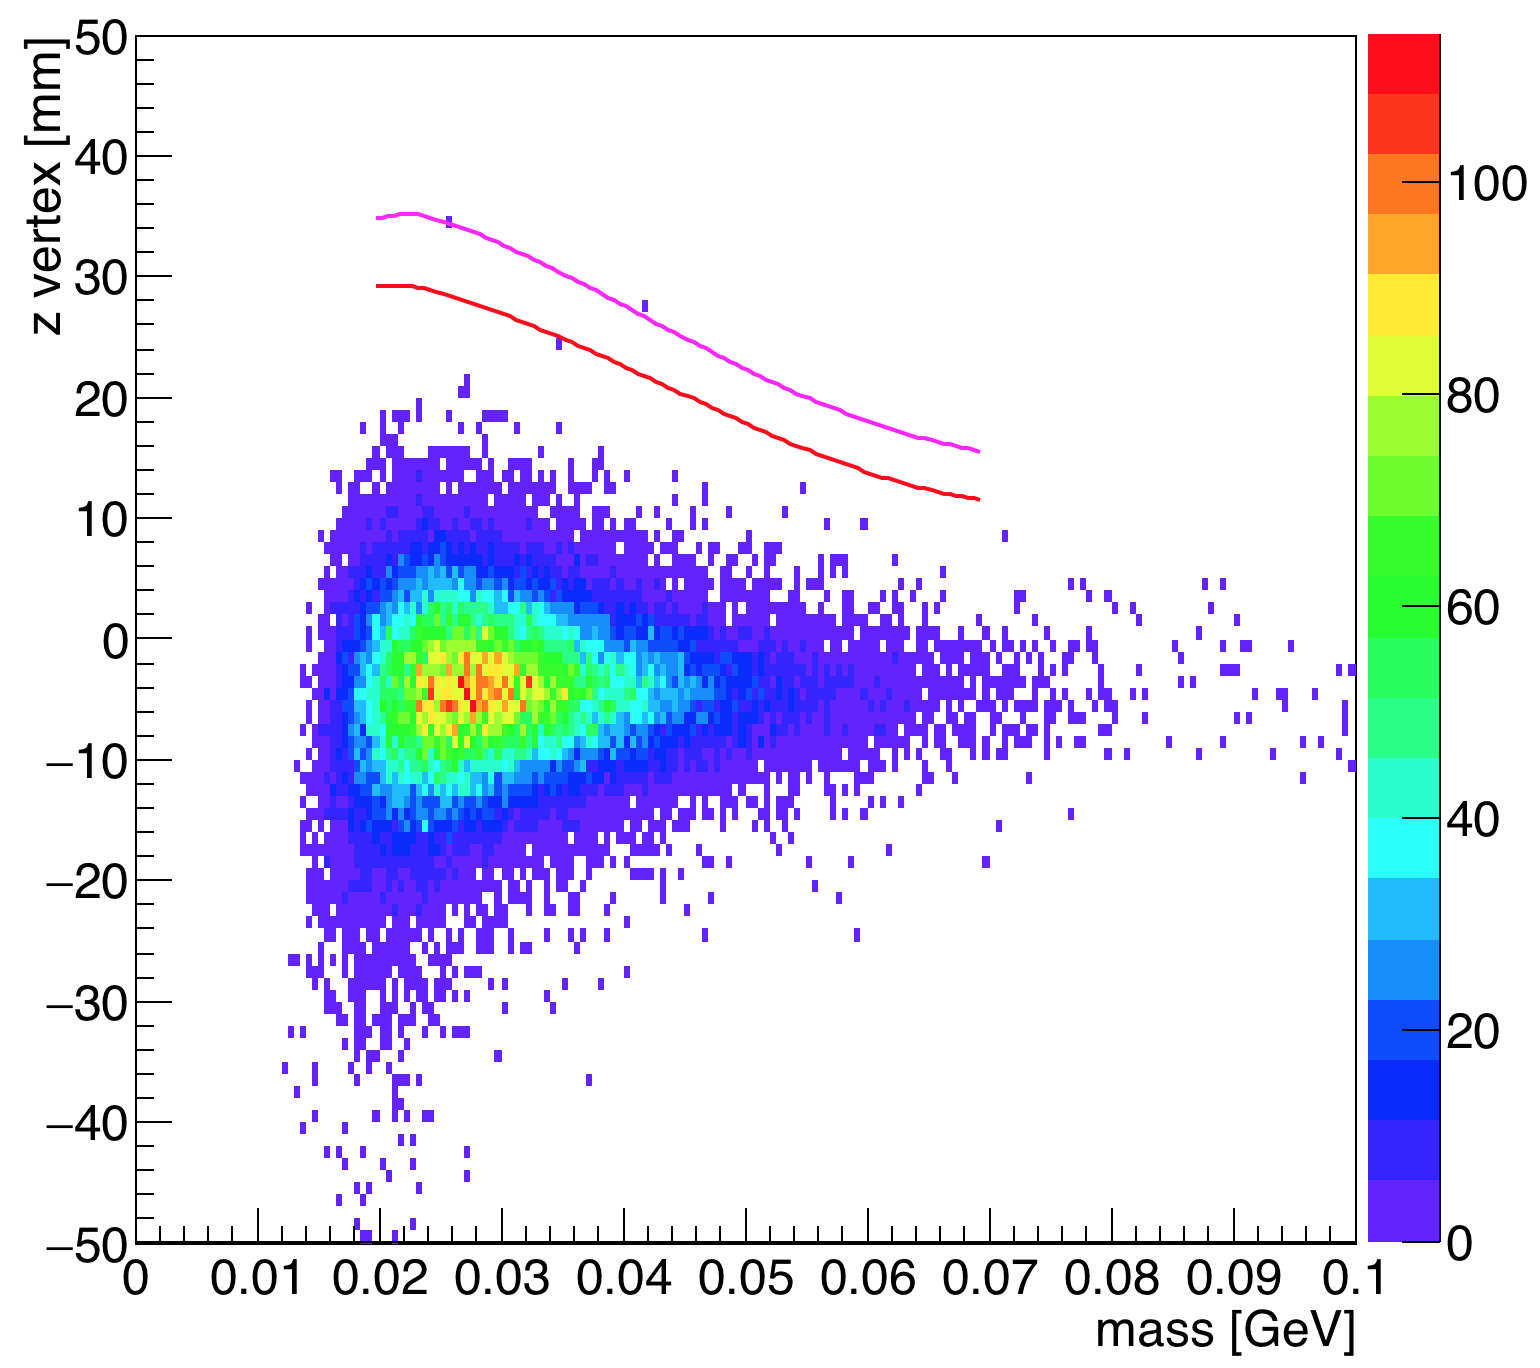
\includegraphics[width=0.75\textwidth]{pics/searching/zVm_acc_L1L1.png}
  \caption[Vertex position vs mass for the 10$\%$ L1L1 accidentals]{The unconstrained $z$ vertex position is shown as a function of the corrected mass of the $e^+e^-$ pair for out of time clusters. These events are selected such that the cluster time difference is greater than 3~ns and less than 9~ns covering a total of six beam buckets. There are three events that contaminate the high $z$ region from accidentals over the six beam buckets. The actual data selection uses clusters from two beam buckets.}
  \label{fig:zVm_acc}
\end{figure} 

In the accidental vertex distribution, we obtained 3 high $z$ events from the selected six beam buckets. The vertex events selected for the vertex search are centered on 2 beam buckets. Therefore, in the 10$\%$ sample, we may have $1\pm0.6$ high $z$ events attributable to accidentals. A rigorous procedure to identify the accidental rate would be to vertex pairs out of time over a large statistical data set. One would expect the effects from the high $z$ background to scale by a factor of 10 to the final full data set. 